\documentclass{article}
\usepackage[utf8]{inputenc}
\usepackage{hyperref}
\usepackage{amsmath}
\usepackage{amsfonts}
\usepackage{graphicx}
\usepackage{enumitem}
\usepackage{wrapfig}
\graphicspath{ {./images} }


\title{IPhO Class - Mechanics}
\author{
    Tan Chien Hao\\
    \texttt{www.tchlabs.net}\\
    \texttt{Telegram @tch1001}
    % new collaborators add your name and contact here!
}

\date{\today}
\begin{document}
\newif\ifpaper

% TOGGLE ANSWER HERE
\paperfalse 

\maketitle
\tableofcontents
\section{Lagrange Multipliers}
Consider the following statics question.
\subsection{Example: 5 Identical Rods}
The figure shows 5 identical uniform rods connected by smooth chains (not shown).
\begin{figure}[h]
    \centering
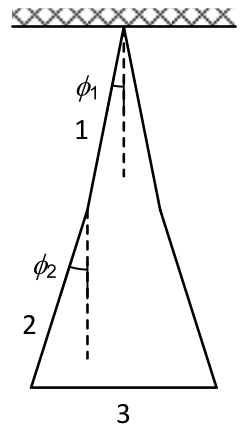
\includegraphics[width=0.4\linewidth]{images/5identicalrods.png}
\end{figure}\\
Determine the angle $\phi_1$ and $\phi_2$.
\subsection{Minimizing GPE}
Let the length of the rod be $L$ and mass be $m$. It is intuitive that the system wants to minimize GPE $E(\phi_1, \phi_2)$ subject to a geometrical constraint. 
\begin{align}
    E(\phi_1, \phi_2) &= 2 mg \left(-\frac{L}{2} \cos \phi_1 \right) + 2mg \left(-L \cos \phi_1 -\frac{L}{2} \cos \phi_2 \right) + mg \left(L \cos \phi_1 + L \cos \phi_2 \right) \notag \\
    &= -2 mgL (2 \cos \phi_1 + \cos \phi_2)  \\
    L &= 2 (L \sin \phi_1 + L \sin \phi_2) \quad \Leftrightarrow\quad \sin \phi_1 + \sin \phi_2 = 1/2
\end{align}
We can use Lagrange multipliers to solve this constrained optimization problem.
\subsection{Lagrange Multipliers}
Lecture
\begin{itemize}
    \item Review multivariate calculus (grad)
    \item Level sets 
    \item Geometrical intuition
    \item Mention Lagrangian mechanics (holonomic constraints)
\end{itemize}
\subsection{5 Identical Rods Solution}
Lecture
\section{Common ODE}
\subsection{$d(v^2)$ integration trick}
Newton's 2nd law is a differential equation for $x(t)$
\begin{align}
    F(t) = m \frac{d^2 x}{dt^2}
\end{align}
\subsubsection{$F(t)$ case}
When $F(t)$ is explicitly known, e.g. $F(t) = F_0 \sin \omega t$, we can integrate both sides with respect to time $t$ to get the impulse-momentum theorem.
\subsubsection{$F(x)$ case}
However, often the force $F(t)$ is dependent on position $F(x(t))$, e.g. $F(x) = -kx$. In such cases, we need to solve an ODE. This can sometimes be easy (e.g. SHM), but in general what we do is integrate with respect to position $x$. This is how we get work-energy theorem and the concept of \textbf{potential energy}. \\[10pt]
Note: Potential energy is only defined for \textbf{conservative} forces.
\subsubsection{$F(v)$ case}
In examples such as linear drag $F(v) = -Av$ or Lorentz force $F(\vec{v}) = e\vec{v} \times \vec{B}$, the equation becomes of the form
\begin{align}
    F(v) = m \frac{dv}{dt}
\end{align}
This is a first order ODE, so we solve for $v(t)$ and integrate to obtain $x(t)$.
\subsubsection{$F(v^2)$ case}
In examples such as quadratic drag $F(v) = -cv^2$, we could theoretically solve the first order ODE like the $F(v)$ case, but this is tedious (you need to integrate $dv/(A+Bv^2)$). You can use the following trick to shortcut the calculations
\begin{align}
    \frac{1}{2} \frac{d(v^2)}{dx} = \frac{dv}{dt}
\end{align}
This is best illustrated using the following example problem.
\subsubsection{Example: Stopping Plane}
A plane landed on a runway with a horizontal velocity of $25 \mathrm{~m} \mathrm{~s}^{-1}$. During taxiing, the plane experienced both drag and lift force of $c_x v^2$ and $c_y v^2$, respectively, where $v$ is the velocity of the plane.\\[10pt]
Suppose $c_x / c_y=0.20$ and the coefficient of friction between the tyres and the runway is $\mu=0.10$, determine the distance the plane travelled on the runway before coming to a stop.
\subsubsection{General Advice}
Pick the appropriate form based on what the question asks
\begin{align}
    \frac{F(t,x,v)}{m} = \frac{d^2x }{dt^2} = \frac{dv}{dt} = \frac{1}{2} \frac{d(v^2)}{dx} 
\end{align}
\subsection{Damped Driven SHM}
Oscillations Video: \url{https://youtu.be/ps-XdLlz80U?t=97}\\[10pt]
We now derive the transient and steady state solution to 
\begin{align}
\ddot{x}+\gamma \dot{x}+\omega_0^2 x&=\frac{F_0}{m} \sin \omega t \\
x&=x_{\text {trans }}+x_{\text {steady }} \\
\ddot{x}_{\text {trans}}+\gamma \dot{x}_{\text {trans }}+\omega_0^2 x_{\text {trans }}&=0 \\
\ddot{x}_{\text {steady}}+\gamma \dot{x}_{\text {steady }}+\omega_0^2 x_{\text {steady }}&=\frac{F_0}{m} \sin \omega t 
\end{align}
Namely, the solution to the transient part (homogeneous solution) is 
\begin{align}
&\ddot{x}_{\text{trans}}+\gamma \dot{x}_{\text{trans}}+\omega_0^2 x_{\text{trans}}=0 \notag \\
&x_{\text{trans}}=e^{-\frac{\gamma}{2} t}\left(A_1 \sin \sqrt{\omega_0^2-\frac{\gamma^2}{4}} t+A_2 \cos \sqrt{\omega_0^2-\frac{\gamma^2}{4} }t\right)\qquad \left(\text { if } \omega_0^2>\frac{\gamma^2}{4}\right) \notag \\
&x_{\text{trans}}=e^{-\frac{\gamma}{2} t}\left(A_1+A_2 t\right)\quad \quad \quad \quad \quad \quad \quad \quad \quad \ \quad \quad \quad \quad \ \qquad \left(\text { if } \omega_0^2=\frac{\gamma^2}{4}\right) \notag \\
&x_{\text{trans}}=e^{-\frac{\gamma}{2} t}\left(A_1 e^{-\sqrt{\frac{\gamma^2}{4}-\omega_0^2 }t}+A_2 e^{\sqrt{\frac{\gamma^2}{4}-\omega_0^2} t}\right) \quad \quad \quad \quad \ \qquad\left(\text { if } \omega_0^2<\frac{\gamma^2}{4}\right) \notag 
\end{align}
And the solution to the steady state part (particular solution) is 
\begin{align}
& \ddot{x}_{\text {steady}}+\gamma \dot{x}_{\text {steady }}+\omega_0^2 x_{\text {steady }}=\frac{F_0}{m} \sin \omega t  \\
& x_{\text {steady }}=\frac{F_0}{m} \frac{1}{\sqrt{\left(\omega_0^2-\omega^2\right)^2+(\omega \gamma)^2}} \sin (\omega t-\phi),& \quad \quad \tan \phi=\frac{\omega \gamma}{\omega_0^2-\omega^2} \notag 
\end{align}
\end{document}